\documentclass[letterpaper, 10pt, oneside]{article}

\newcommand\tabref[1]{Tab.\,\ref{#1}}
\newcommand{\fakepar}[1]{\vspace{0.5mm}\noindent\textbf{#1.}}

\usepackage[hmargin=1in,vmargin=0.9in]{geometry}
\usepackage{geometry}
\usepackage{graphicx}
\usepackage{caption}
\usepackage[labelformat=simple]{subcaption}

\renewcommand{\thesubfigure}{Figure \arabic{subfigure}:}

\begin{document}

\newgeometry{margin=2cm}
\begin{titlepage}
    \begin{center}
        \large
        \textbf{POLITECNICO DI MILANO}\\
        Scuola di Ingegneria Industriale e dell’Informazione\\
        Dipartimento di Elettronica, Informazione e Bioingegneria\\
        \vspace{0.4cm}
        \begin{figure}[!h]
            \begin{center}
                
\includegraphics[width=0.35\columnwidth]{logo_polimi.png}
            \end{center}
        \end{figure}

        \vspace{10mm}

        \huge\textbf{DIGITAL DESIGN OF EMBEDDED SYSTEMS IN THE IOT AND RISC-V OPEN CORE ERA}

        \vspace{25mm}

        \LARGE\textbf{COURSE PROJECT REPORT}

        \vspace{15mm}

        \LARGE\textbf{SystemVerilog implementation of the\\Salsa20 stream cipher}

        \vfill
        \hfill
        \begin{tabular}[t]{r@{}}
            Andrea Maioli\\
            Student ID n. 938144\\
            Academic Year 2020-2021
        \end{tabular}
    \end{center}
\end{titlepage}
\restoregeometry


\begin{figure}[!t]
    \begin{subfigure}[c]{0.5\textwidth}
        \centering
        \resizebox{\textwidth}{!}{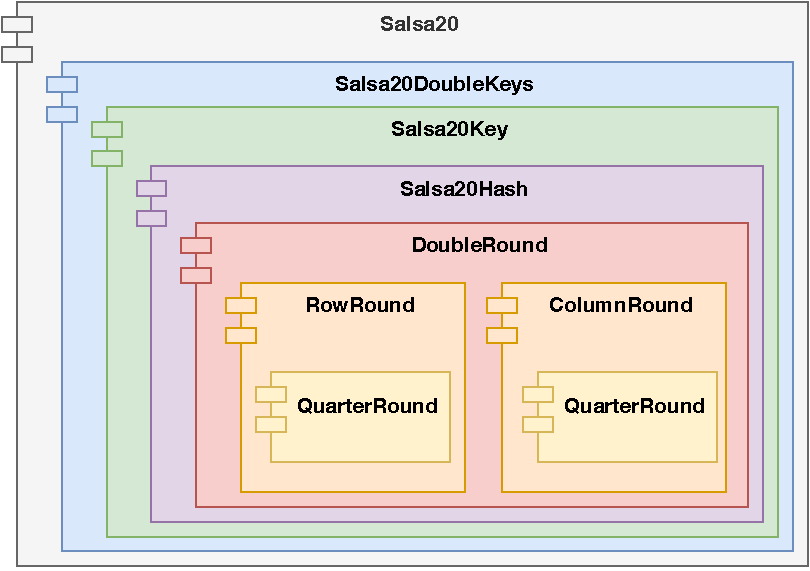
\includegraphics{figure.pdf}}
        \caption{Salsa20 modular architecure}
        \label{fig:architecture}
    \end{subfigure}
    \begin{subfigure}[c]{0.5\textwidth}
        \centering
        \resizebox{0.85\textwidth}{!}{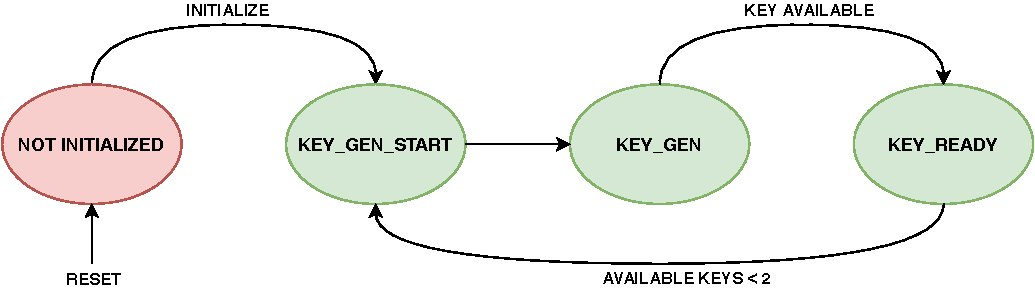
\includegraphics{fsm.pdf}}
        \caption{Salsa20DoubleKeys simplified FSM}
        \label{fig:fsm}
    \end{subfigure}
\end{figure}

\section{System Overview}
This project consists in a digital design of the Salsa20 stream cipher~\cite{salsa20}.
The key feature of the Salsa20 stream cipher resides in its key expansion algorithm, which generates an unique key starting from from a given key and nonce.
The generated key is then used as the key of a One Time Pad, which applies the XOR operator to the input plaintext (ciphertext) and the generated key to output the corresponding ciphertext (plaintext).

We divide our design of the Salsa20 stream cipher into a modular architecure that reflects the same logical division of the Salsa20 algorithm.
Fig.\,1 shows the modules that compose our architecture.
In the following sections we describe the functionality of these modules and how they interact with each other.

\subsection{Key Generation}
The \textbf{Salsa20Key} module generates the key necessary for the encryption or decryption of a given block of data.
This module takes as input the clock and reset signals, a start signal, a 4 bits rounds signal, a keylength signal, a 32 bytes key, a 8 bytes nonce, and a 8 bytes block identifier, and it outputs a valid signal and the generated key.
The Salsa20Key module uses combinatorial logic to expand the input key and nonce onto a 64 bytes squared matrix.
The keylength signal decides if we need to consider all the 32 bytes of the key, or only the first 16 bytes, as the Salsa20 algorithm supports keys of both 16 and 32 bytes.
Then, the Salsa20Key module forwards the generated matrix, the clock and reset signals, the rounds signal, and the start signal to the \textbf{Salsa20Hash} module, which transforms the matrix.

The Salsa20Hash module applies multiple times a given set of transformations to the input matrix.
Our design supports different variants of the Salsa20 stream cipher, which differ only in the number of transformation rounds $n$ that they apply to generate the key.
Such number is specified by the rounds signal.
Note that $n$ is $10$ for Salsa20, $6$ for Salsa12, and $4$ for Salsa8.

Each round applies the Salsa20' \textit{doubleround} function to the matrix, which transform each row and column using the \textit{quarterround} function.
We implement this functionality in the \textbf{DoubleRound}, \textbf{RowRound}, \textbf{ColumnRound}, and \textbf{QuarterRound} modules.
The core logic of these modules stands inside the QuarterRound module, which applies combinatorial logic to a given set of inputs, consisting in an entier row or column of the input matrix.
Then, both the RowRound and ColumnRound rely on the QuarterRound module to apply the corresponding transformation.
The RowRound (ColumnRound) module instantiates 4 QuarterRound modules, one for each row (column).
The DoubleRound module acts as a logical container that takes the input matrix, sends it to the RowRound module, collects the resulting matrix, sends the transformed matrix to the ColumnRound module, and finally outputs the resulting matrix.
This module represents the critical path of the implementation and takes $20ns$ to transform the input matrix.

The Salsa20Hash module instantiates a single DoubleRound module and applies one matrix transformation at each clock cycle, by feeding the DoubleRound module with the result produced during the previous clock cycle.
Note that the transformation starts upon receiving the start signal and ends after $n$ rounds.
When the last round executes, the Salsa20Hash module sums the original matrix and the transformed matrix, and outputs the result, alongside with a valid signal.
Note that this data is forwarded back to the Salsa20Key module and represents also its output.

\subsection{Key Buffer}
The Salsa20 algorithm uses a 64 bytes key to encrypt or decrypt a 64 bytes sequence of data, and a block identifier is incremented every 64 bytes to expand a new key, starting from the initial key and nonce.
Being Salsa20 a stream cipher, we can generate beforehand the key for encrypting (decrypting) the next sequences of data, as it does not depends on the previously encrypted (decrypted) data.
This allows us to generate the next key while we are encrypting (decrypting) the current sequence of data, with a consequent increase of system performance, as we need not to wait for the next key when we reach the end of a 64 bytes sequence.

For this reason, we implement the \textbf{Salsa20DoubleKeys} module, which constantly generates a new key and saves it onto a circular buffer that stores up to two keys.
In addition to the same inputs of the Salsa20Key module, this module takes as input an init signal and a next\_chunk signal, and outputs an initialized signal, a ready signal, a valid signal, and a 8 bytes key chunk.
Note that the module outputs a ready signal whenver the circular buffer is not empty, and splits each key into 8 chunks of 8 bytes each.
Whenever the circular buffer is not empty and the module receives a next\_chunk signal, it outputs the first unused 8 bytes of the key that is on top of the circular buffer.

The Salsa20DoubleKeys module exploits a FSM to buffer and generate new keys, for which Fig.\,2 shows a simplified state diagram.
The module starts in the \textit{NOT\_INITIALIZED} state.
When it receives the init signal, it initializes the block identifier and the circular buffer, and then it moves to the \textit{KEY\_GEN\_START} state.
Here it signals an instance of the Salsa20Key module to generate a new key, and then it moves to the \textit{KEY\_GEN} state, where it waits for the generated key.
Once the Salsa20Key module outputs a key, the Salsa20DoubleKeys module saves it onto a buffer, increments the buffer index and the block identifier, and it moves back to the \textit{KEY\_GEN\_START} state.
Note that such action happens only if the key buffer is not full, that is, if the number of available keys is lower than $2$.

\subsection{Encryption and Decryption}
The Salsa20 encryption and decryption functions use the same logic, as they both rely on the XOR operator, which is an involutory function.
We implement this logic inside the \textbf{Salsa20} module, which takes as input the clock and reset signals, an init signal, a data encrypt/decrypt signal, a write enable signal, a 2 bits address, and a 8 bytes input signal.
The Salsa20 module stores the 32 bytes key, the 8 bytes nonce, the number $n$ of rounds, and the keylength onto dedicated registers.
To setup these registers, we need to split such data into chunks of 8 bytes each and provide them across multiple clock cycles as input signals, alongside with the write enable signal and the corresponding address of the chunk.
Once we provide all the necessary data, we need to initialize the module using the init signal.

The Salsa20 module contains an instance of the Salsa20DoubleKeys module and forwards to it the init signal.
These two modules outputs the same ready signal, meaning that the Salsa20 module is ready to encrypt or decrypt an 8 byte input whenever a key is available.
When the Salsa20 module is ready, we need to set the data encrypt/decrypt signal and provide 8 bytes of data as input.
Then, the Salsa20 module retrievers a key chunk of 8 bytes from the Salsa20DoubleKeys module and XORs the key chunk with the input data, providing the encrypted (decrypted) result as output, alongside with a valid bit.

\begin{table}[!t]
    \centering
    \begin{tabular}{|c|c|c|c|}
        \hline
        ~ & \textbf{Synthesis} & \textbf{Implementation}\\
        \hline
        \textbf{LUTs} & 2586 ($4.08\%$) & 2582 ($4.07\%$)\\
        \hline
        \textbf{Slice Registers} & 2590 ($2.04\%$) & 2590 ($2.04\%$)\\
        \hline
        \textbf{F7 Muxes} & 128 ($0.40\%$) & 128 ($0.40\%$)\\
        \hline
        \textbf{F8 Muxes} & 64 ($0.40\%$) & 64 ($0.40\%$)\\
        \hline
        \textbf{IOB Ports} & 139 ($66.19\%$) & 139 ($66.19\%$)\\
        \hline
        \textbf{BUFGCTRL Clock} & 2 ($6.25\%$) & 2 ($6.25\%$)\\
        \hline
    \end{tabular}
    \caption{Resource utilization and performance of the implemented design.}
    \label{tab:results}
\end{table}

\section{System Performance}
We validate our design using both the example data provided in the Salsa20 whitepaper~\cite{salsa20} and a python implementation of the Salsa20 algorithm.
We test the Salsa20, Salsa12, and Salsa8 versions using both 32 bytes and 16 bytes keys.

We synthesize and implement the design of the Salsa20 stream cipher using as target device the Xilinx Artix 7 model \textit{7a100tcsg324-1}.
Tab.\,1 shows the resource utilization of our design, both after the synthesis and the implementation steps.
The Salsa20DoubleRound is responsible for most of the LUTs utilization, as it requires $2136$ LUTs both after the synthesis and implementation.
Instead, the Salsa20DoubleKeys module is responsible for most of the registers utilization, as it requires $2200$ registers, which uses to store the two keys.
Note that the Salsa20Key module uses $1096$ slice registers to provide a single key to the Salsa20DoubleKeys module.
Similarly, the Salsa20DoubleKeys module uses all the F7 and F8 muxes that our design occupies.

\fakepar{Timing and throughput}
We execute the timing analysis of our designs, identifying that the minimum clock period is $23.33ns$, that is, a maximum clock frequency of $43.33$\textit{MHz}.

Our Salsa20Key module requires $n$ clock cycles to generate a key, with $n$ equal to the number of rounds of the Salsa20 version adopted.
Our Salsa20DoubleKeys module requires $n+2$ clock cycles for its initialization and for the generation of the first key. 
When a burst of key chunk requests consumes the $8$ chunks of the first generated key, the Salsa20DoubleKeys requires $4$ clock cycles to generate a new key when the burst ends when the number of rounds is $10$, that is, the Salsa20 version.
Note that in the Salsa12 (Salsa8) version, that is, $n = 6$ ($n = 4$), the Salsa20DoubleKeys module requires no extra clock cycles to generate the second key, as it is always ready before the last chunk of the previous key is requested.

Finally, we need $6$ ($4$) clock cycles to set up the Salsa20 module, as it requires $1$ clock cycle to set up the keylength and the number of rounds, $4$ ($2$) clock cycles to set up the $32$ ($16$) bytes key, and $1$ clock cycle to set up the $8$ byte nonce.
For the initialization and the key generation requires the same clock cycles of the Salsa20DoubleKeys module.
Our Salsa20 module introduces $1$ clock cycles delay to generate the ciphertext (plaintext) of an input plaintext (ciphertext).
After the first request, it is able to output a ciphertext (plaintext) at every clock cycle, if the key is ready.

\bibliographystyle{abbrv}
\bibliography{bibliography}

\end{document}
